\chapter{Implementación de bloques del sistema}
\label{sec:implementacion_bloques_sistema}

%COMENTARIO: ACÁ SE ME OCURRE DE HACER UNA INTRODUCCIÓN A CADA BLOQUE DEL SISTEMA, JUSTIFICAR Y EXPLICAR MEDIO POR ARRIBA Y EN LAS SIGUIENTES SECCIONES EXPLICAR LOS DETALLES MÁS TÉCNICOS DE CADA BLOQUE.

En base a lo estudiado en la etapa de investigación, se pudo concluir que un sistema de captura de movimiento con las características necesarias para cumplir el objetivo del proyecto debe estar formado por 4 bloques generales: \emph{calibración}, \emph{detección de marcadores}, \emph{reconstrucción} y \emph{seguimiento}. En la figura \ref{bloquesSist} se muestra un esquema del sistema a implementar.

\begin{figure}[ht!]
\hspace{-0.5cm}
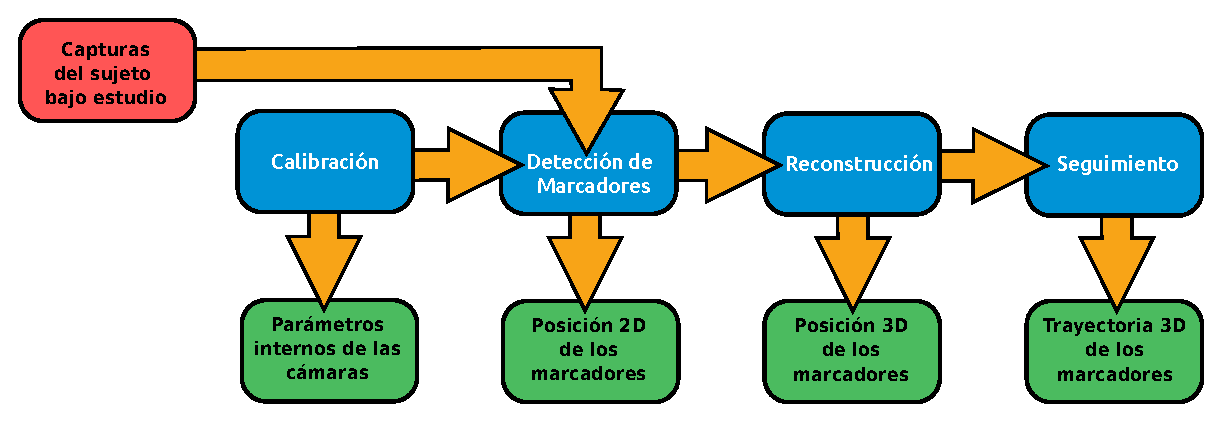
\includegraphics[scale=0.7]{img/Sistema_completo/Diagrama_de_bloques.eps}
\caption{Diagrama de bloques del sistema completo.}
\label{bloquesSist}
\end{figure}

A grandes rasgos, el sistema funciona de la siguiente manera:

\begin{enumerate}
	\item Se \emph{calibran} las cámaras. Esto es, determinar los parámetros de las mismas de forma tal de tener un mapeo del espacio 3D a las coordenadas 2D de las imágenes capturadas.
	\item Se realiza la captura del paciente en movimiento desde todas las cámaras calibradas.
	\item A partir de las secuencias, se realiza la \emph{detección de marcadores} para cada cámara. Esto equivale a determinar la posición 2D de dichos marcadores en cada cámara donde están visibles, a lo largo de toda la secuencia.
	\item Luego, con la posición 2D de determinado marcador en al menos 2 cámaras se realiza la \emph{reconstrucción} del mismo, es decir, obtener las coordenadas 3D de dicho marcador. Se realiza para todos los marcadores, y para todos los cuadros de la secuencia.
	\item Finalmente, se realiza el \emph{seguimiento} (o \emph{tracking}) de cada marcador en el espacio. Con esto se obtienen las trayectorias 3D de todos los marcadores en el cuerpo del paciente.
\end{enumerate}

Debido a los tiempos disponibles para realizar el proyecto en su totalidad, y junto a la planificación realizada al comienzo del mismo, se tiene como idea principal el conseguir la implementación de un sistema con características similares, adaptando el mismo para cumplir los objetivos establecidos. 

Sin embargo en la investigación bibliográfica se encuentra otra realidad, puesto que no hay muchos sistemas a disposición. Por un lado, la mayor parte de los sistemas encontrados poseen altos costos de licenciamiento (por ejemplo Vicon \cite{vicon}, OptiTrack \cite{optitrack}, PhaseSpace \cite{phasespace}, Qualisys \cite{qualisys} o MotionAnalysis \cite{motion_analysis}) y por otro lado, los sistemas de código abierto no se adaptaban a las necesidades presentes o el trabajo a realizar sobre los mismos era más Costoso que hacer una implementación propia. En este último caso se encuentra el software Kinovea \cite{kinovea}, que realiza únicamente el seguimiento en coordenadas 2D.

Debido a los inconvenientes planteados, se decide realizar una implementación propia de los bloques del sistema. Nuevamente, de acuerdo a la filosofía explicada en los párrafos anteriores, se prioriza la búsqueda de sistemas ya implementados cuyo diseño se corresponda a cada bloque de la Figura \ref{bloquesSist},  antes de recurrir a la creación de uno.

Se tuvo presente en esta búsqueda el hecho de poder separar el sistema en bloques independientes. Esto asegura que la construcción de uno de ellos no dependa del correcto funcionamiento de otro. Por otro lado, da la posibilidad que en etapas futuras se pueda realizar el estudio de uno de los bloques de la Figura \ref{bloquesSist} individualmente y así poder modificarlo u optimizarlo sin afectar al resto. Esta forma de trabajo funciona adecuadamente siempre y cuando la salida de un bloque sea exactamente la entrada del siguiente, para los casos en que no se logra esto, se realizan algoritmos capaces de importar la salida de un bloque y convertirla al formato de entrada de otro (por ejemplo, \textit{Xml2Struct} que convierte el xml que tiene como salida el bloque de detección de marcadores en estructuras de Matlab para realizar la reconstrucción).

Como se menciona anteriormente, en la búsqueda realizada se encuentra la tesis de doctorado de Lorna Herda\cite{herda}, la misma plantea un sistema de captura de movimiento con las características buscadas para este proyecto. Al estudiar dicho sistema se encuentra que posee las mismas hipótesis de uso que el estudio preliminar realizado (utilización en fisioterapia, biomecánica, animación, deporte, etc.). Además, es un trabajo mencionado repetidas veces en otros artículos de la misma rama científica, encontrándose una documentación amplia respecto a la metodología implementada.

Debido a las ventajas que presenta esta metodología respecto a las otras encontradas, se decide implementar el sistema de Herda y elaborar los bloques de calibración y detección de marcadores aparte.

Estudiado el diseño propuesto por Herda para su sistema, se construye un diagrama de bloques completo, más detallado que el mostrado en la Figura \ref{bloquesSist}, el cual se puede observar en la Figura \ref{diagBloq}. Es importante destacar que, si bien la mayor parte de los bloques de reconstrucción y seguimiento se realizaron con la metodología del sistema de Lorna Herda\cite{herda}, en la documentación se presentan ciertas ambigüedades respecto a la descripción de algunos métodos y en la forma de resolver determinados casos de uso, que tuvieron que ser analizados y definidos por el grupo del proyecto en base a los conocimientos adquiridos.

A continuación se muestra el diagrama de bloques y se explica su funcionamiento.

\section{Diagrama de bloques}

\vspace{-0.5cm}
\begin{figure}[ht!]
\hspace{-1cm}
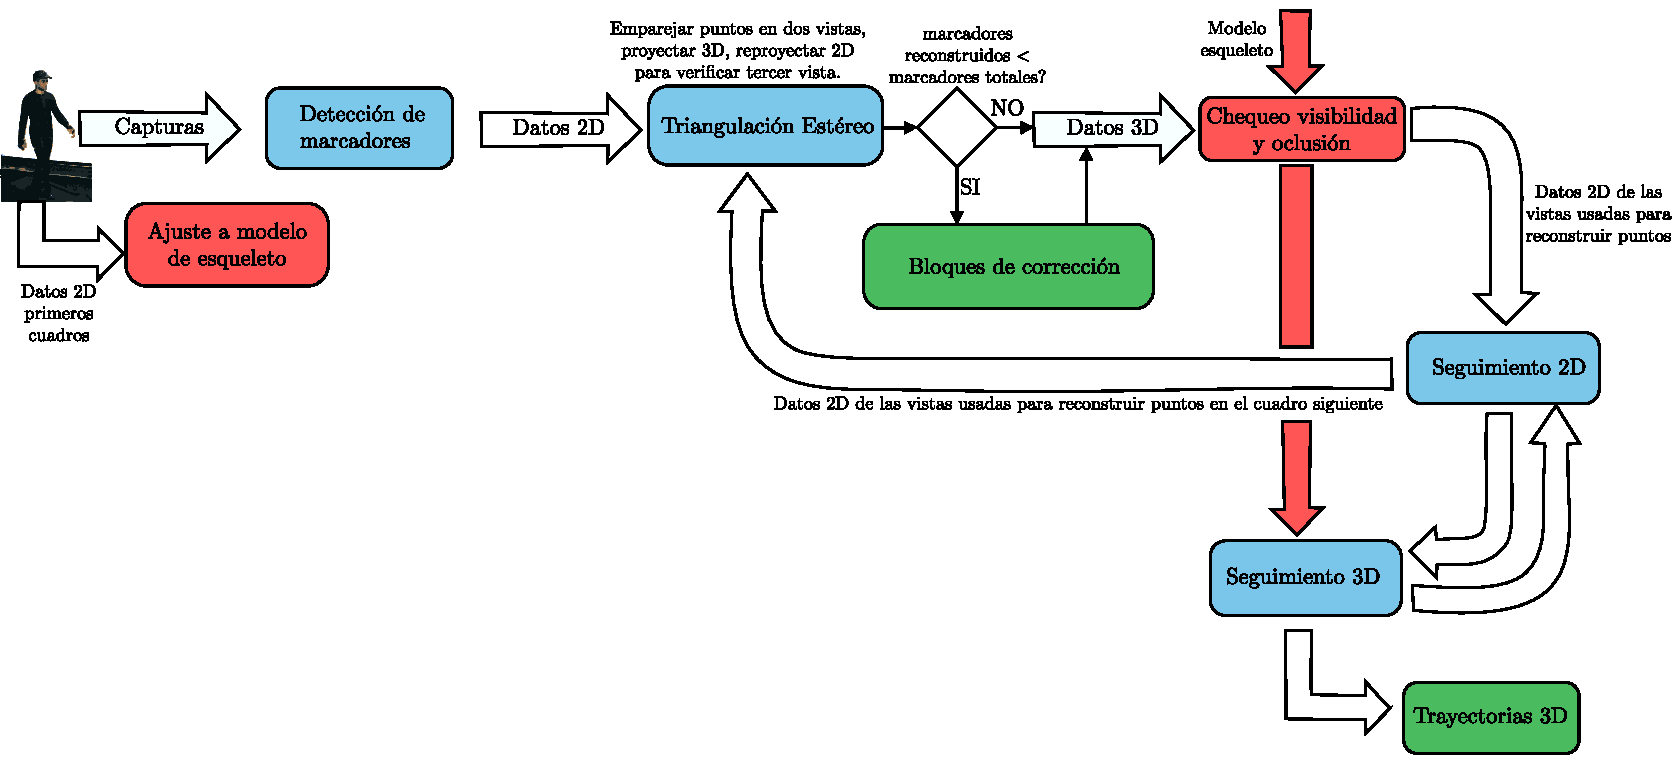
\includegraphics[scale=0.55]{img/Sistema_completo/Diagramadebloques_Herda.pdf}
\vspace{-1cm}
\caption{Diagrama de bloques detallado del sistema.}
\label{diagBloq}
\end{figure}

El sistema representado en este diagrama, funciona de la siguiente manera:

\begin{enumerate}
\item Se realiza la captura de movimiento del paciente desde múltiples vistas, en un entorno controlado. Estas capturas son la entrada principal al sistema.
\item A partir de las capturas, por un lado se ajusta el \textbf{modelo teórico de esqueleto} a utilizar, de acuerdo a las características del cuerpo del paciente, y por otro lado se realiza la \textbf{detección de marcadores} de cada cuadro para cada cámara. Este bloque es el mismo que el del diagrama de la figura \ref{bloquesSist} y se explicará en detalle en el Capítulo \ref{deteccionMarcadoresSec}.
\item Luego que se tiene la posición 2D de los marcadores en cada cuadro y en cada cámara, se realiza la \textbf{triangulación estéreo} para obtener la posición 3D de los mismos. A grandes rasgos, la \emph{triangulación 3D} empareja dos puntos en correspondencia de dos vistas distintas y con ellos calcula la proyección 3D de ese punto en el espacio, luego se re-proyecta ese punto en las otras vistas para verificar. Si verifica su posición en al menos una vista más, entonces la posición 3D se considera válida.
\item Si el número de marcadores reconstruidos en 3D es menor al número total de marcadores en el modelo de captura, se ingresa en el \textbf{bloque de corrección}, donde se utilizan varios métodos para recuperar la posición 3D de los marcadores restantes (ver Figura \ref{fig:bloqCorr}). 
\item Cuando se tiene la posición 3D de todos los marcadores, se ingresa en el bloque de \textbf{chequeo de visibilidad y oclusión} donde se verifica que la posición reconstruida de cada marcador sea correcta y no se haya reconstruido alguno con datos erróneos.
\item Finalmente, se realiza el \textbf{tracking 3D y 2D} en simultáneo para reconstruir las trayectorias de cada marcador.
\end{enumerate}

La explicación detallada de cada bloque y cómo fueron implementados se muestra en los capítulos siguientes.

A continuación, se explica como funciona el bloque de corrección:

\begin{figure}[ht!]
\hspace{-1cm}
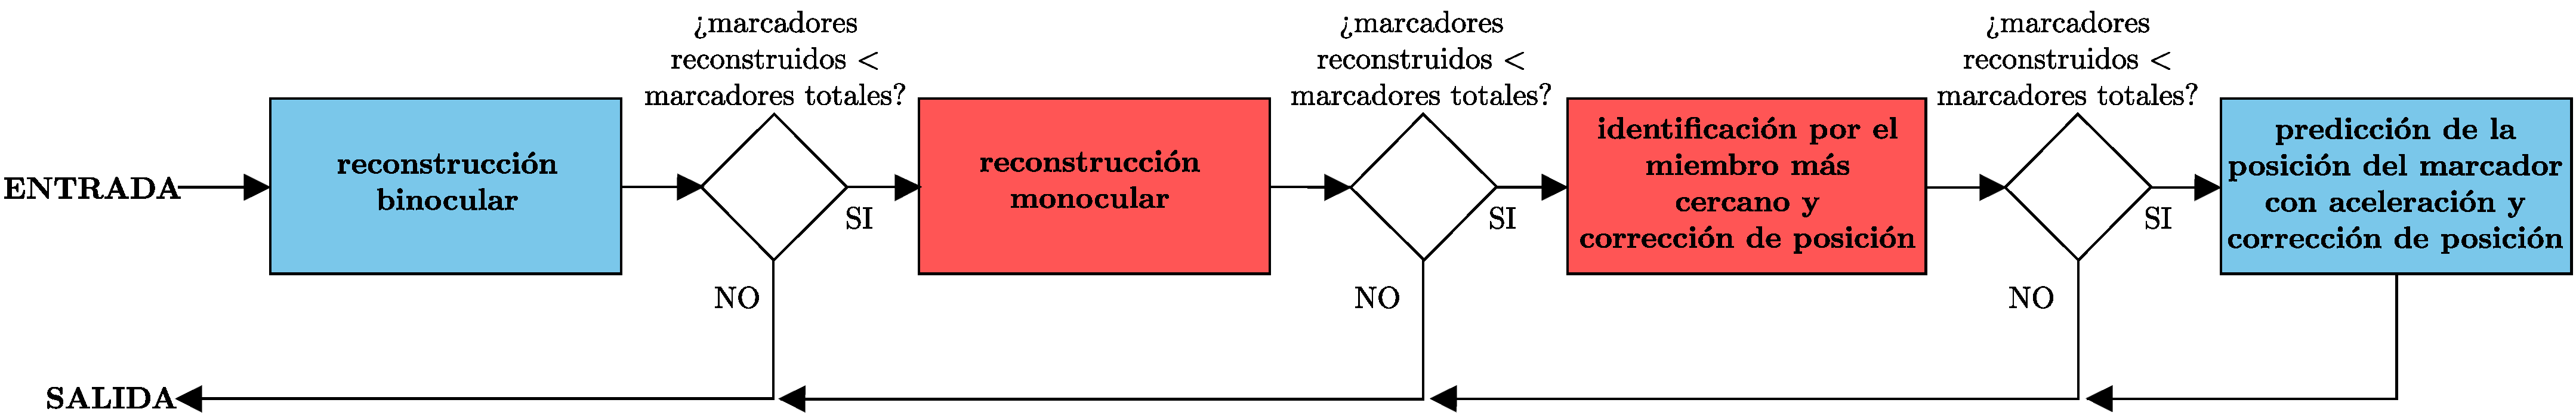
\includegraphics[scale=0.22]{img/Sistema_completo/BloquesDeCorreccion}
\caption{Detalle del bloque de corrección.}
\label{fig:bloqCorr}
\end{figure}

Una vez realizada la triangulación estéreo, se verifica que el número de marcadores reconstruidos sea igual a la cantidad de marcadores que efectivamente se estén usando en la adquisición de datos. Si esta condición no se verifica, se ejecuta un “bloque de corrección” para solucionarlo. Dicho bloque a su vez, contiene  varios sub-bloques, los cuales pueden verse en la figura \ref{fig:bloqCorr}.

Primeramente se efectúa la \emph{reconstrucción binocular} y si aún no se obtienen todos los marcadores se efectúa la \emph{reconstrucción monocular}, se disminuye la exigencia sobre la reconstrucción al utilizar sucesivamente métodos menos precisos, con el fin de completar el número de \emph{marcadores reconstruidos}.

 Si en la salida de cada uno de los bloques anteriores la condición de \emph{todos los marcadores reconstruidos} aún no se cumple, se pasa al siguiente bloque, donde se asocian los marcadores 3D reconstruidos que aún no fueron identificados con aquellas articulaciones del modelo de esqueleto (ajustado en la inicialización) que no tienen ningún marcador asociado. Para esto, se evalúan las distancias de los marcadores no identificados con la posición de las articulaciones del modelo en cuadros anteriores y se asocian aquellos marcadores que se encuentren a menor distancia a cada una de dichas articulaciones. Al tiempo que se realiza esto, se verifica que la distancia entre marcadores asociados a un mismo hueso del esqueleto se mantenga aproximadamente constante (dado que los marcadores están fijos en los huesos y los mismos no varían su tamaño).
 
Si aún faltan marcadores sin reconstruirse, se utiliza como último recurso la estimación de la posición del marcador evaluando la aceleración del mismo en cuadros anteriores y verificando que dicha estimación sea coherente con el modelo de esqueleto.



Si bien se intentó reproducir el sistema propuesto por Herda\cite{herda} tal cual se especificaba en su documentación, se presentaron diversos obstáculos que impidieron poder implementar los bloques de reconstrucción y seguimiento como se detallan anteriormente. Un obstáculo importante son las ambigüedades presentadas en las especificaciones de los bloques en la documentación de Herda, dado que retrasaron la etapa de estudio del sistema al tener que investigar e implementar métodos para poder superar los vacíos presentes en la teoría. Esto último junto con la gran cantidad de módulos a implementar y el tiempo con que cuenta este proyecto generaron diferencias con lo propuesto por Herda.

 A raíz de esto, se decide dar prioridad a los bloques principales del diagrama frente a los secundarios o a los que se implementan para casos de uso particulares. Con esto se intenta tener implementado un sistema de principio a fin, capaz de capturar la posición 3D de un sujeto realizando el movimiento de marcha a lo largo del tiempo con una performance aceptable. Estos bloques son:
 \begin{itemize}
 	\item Detección de marcadores
 	\item Triangulación estéreo (Reconstrucción)
 	\item Seguimiento 3D
 	\item Calibración
 \end{itemize}

En los capítulos que siguen, se explicará el funcionamiento de estos bloques de forma detallada, así como su implementación y el análisis de resultados de cada uno de ellos.